\section{Graphics Card Simulations}

\par
The probabilistic approach described in \autoref{sec:s2lightmap} provides a significant performance improvement over simulating each photon individually. 
However, there are several significant factors which limit the feasibility of using similar methods for the rest of the detector, including:
\begin{itemize}
    \item Optical propagation being required to be performed at least once
    \item Other regions of the detector containing significantly more complex geometry
\end{itemize}
For example, if a probabilistic map were to be applied to the entire TPC liquid xenon region, several weeks' worth of a full computing cluster would be required to produce the equivalent statistics.
Although there are ways in which this could be reduced - such as Z-line symmetry - the initial overhead remains impractically high.
Additionally, the computing cost\footnote{cost in terms of time and computing memory} of looking up the results are likely to mitigate any gain, so are not necessarily faster than just simulating them.
This motivates looking for a different approach.

\subsection{Geant4 Simulations}
\par
Before attempting to improve the speed of simulation, it is important to understand why simulation speed is limited. 
LZ particle propagation simulations are performed in BACCARAT, a software package built upon GEANT4.
In GEANT4, a detector is defined by solid-based modelling or Constructed Solid Geometry (CSG) \cite{geant4_geometry_ref}.
A detector (or scene) is defined by a set of primitive volumes that can be described by some parameters.
An example of this is a sphere; a primitive solid that can be described by a single parameter; radius.
Primitives can be rotated, displaced and combined with other primitives via boolean operations to create more complex solids such as that shown in \autoref{fig:csg_geometry_example}.
\begin{figure}
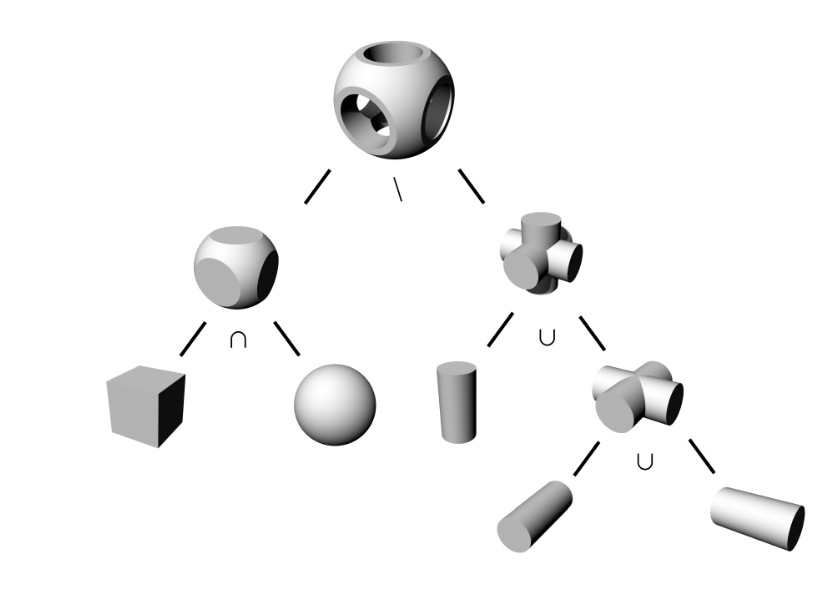
\includegraphics[height=8cm]{Figures/Simulations/csg_geometry.png}
\centering
\caption{Complex solid created from 5 primitive solids using boolean operations; union $\cup$, intersection $\cap$ and difference \textbackslash. Adapted from \cite{csg_geomtry_ref}}
\label{fig:csg_geometry_example}
\end{figure}

\par
In application, the primitive is defined by more than the basic shape parameters (such as radius).
The parameters are used in combination with functions so properties of the solid can be retrieved.
For example, the solid must be implemented in such a way that it is possible to determine if a point $\vec{x}$ is within the solid, and whether a ray travelling in direction $\hat{d}$ will intersect with the surface of the solid.
These functions have to account for all relevant calculations that relate to a solid.
\par
All of the solids in a scene are contained within a geometry tree.
The top of the tree contains the `world' volume, inside which there are daughter volumes (which do not overlap with each other).
These volumes can contain their own daughters, and so on.
To the user, this structure is often less obvious with solids connected to each other by logical volumes (LV) and physical volumes (PV).
LVs contain information associated with a solid such as material. 
PVs can contain one or more LV which are given positions and rotations inside of it. 
A PV can be part of a higher-up LV.
\par
When a particle is simulated, its track starts inside a volume of a solid which is in the geometry tree.
In the direction of travel, a check must be performed to determine intersections with the volume as well as all immediate daughter volumes.
As each daughter is a subtraction in volume of its parent, the number of possible interactions is generally limited.
Even so, the number of sibling volumes is often a reliable indicator of particle tracking performance.
Therefore it is logical for the tree to be as narrow as possible to reduce the number of sibling volumes.
This can be at odds with how a detector is designed, such as if a solid has to have holes for other solids to pass through.
The problem with this is that the interior of the solid is no longer fully defined by the volume\footnote{An example of this in LZ geometry are the calibration tubes, passing through the water tank, outer detector, and OCV}.
In this case, the geometry tree is widened so that volumes inside become siblings of the problem volume, which in turn increases the number of intersection calculations.
This must be the case to enforce the requirement that each volume is contained entirely by its mother volume and that it does not overlap with siblings.
\par
GEANT4, in part, mitigates this by separating the geometry tree nodes into perpendicular facing boxes, called voxels \cite{geant4_voxel_ref} which are not part of the detector volumes.
During particle propagation, the voxels are first checked for intersections.
If there is an intersection, the detector volumes contained within that voxel are then checked.
Though useful, the voxels are limited to a single tree level, with the check performed iteratively (1 axis at a time) to save memory and so can decrease the simulation speed.
The GEANT4 approach can be summarised as:
\begin{quote}
    A detector is a tree of nested solids, each composed of some material and mathematically implemented by a particular C++ class.
\end{quote}

\subsection{Optical Simulations}
\par
In addition to particle tracking, GEANT4 must also handle particle interactions inside a volume which can result in daughter particles that also need to be tracked.
However, in LZ the bottleneck is in the photon propagation, taking up in excess of 95\% of computing time (after using the S2 Light Map).
Optical photon simulations are relatively simple in that no daughter particles need to be tracked.
There is some probability of a photon being absorbed and re-emitted during propagation, but otherwise, photon propagation can be simplified to travelling in a straight line until they reach a boundary.
The simulation is therefore dominated by intersection calculations, or ``\textit{has the photon reached the edge of this volume yet?}".
Therefore increasing the number of these calculations that can be evaluated per second will decrease the overall simulation time.
\par
GEANT4-based simulations are performed on CPUs which have typically been designed to minimise task latency; i.e. the time required to complete any given task.
Although it is possible to multi-thread simulations, it is rarely done due to simulation frameworks often originating decades ago.
An alternative processor widely available is a GPU, which is designed to maximise throughput.
This is achieved by having individual poorer thread performance but by having more threads available\footnote{Additionally, each task should be as independent as possible and require very few resources}.
If a simulation can be moved onto a GPU it will allow for more concurrent tasks that will massively outweigh the slower performance of each task, resulting in more intersection calculations per second.
\par
There have been many different attempts to transfer parts of or entire simulations onto GPUs, such as Chroma \cite{chroma_whitepaper_ref}, ANTS2 \cite{ants2_whitepaper_ref}, Exascale Computing Project \cite{ExaSMR_whitepaper_ref} and MPEXS \cite{mpexs_whitepaper_ref}.
The majority of these make use of NVIDIA CUDA \cite{cuda_ref}, an application programming interface (API) allowing for GPU hardware to be used for general-purpose computing.
%[TODO XXX Geant4 VecGeom]
\par
Chroma is of particular interest as it was proposed and designed for optical simulations and it has been utilised in several experiments \cite{chroma_with_tpcs1_ref,chroma_with_tpcs2_ref,chroma_with_tpcs3_ref}, and has more recently received attention by 3rd generation direct detection dark matter experiments \cite{DARWIN_GPU_simulations_2022_ref}.
Chroma uses surface-based modelling where a triangle mesh describes the geometry.
This tessellation reduces the number of primitives to one, a triangle, which is defined within CUDA programs written by the user.
As the surface of a solid is described by a finite set of triangles, this naturally leads to curves not being represented as accurately as the GEANT4 method.
To some extent, this can be mitigated by increasing the density of the primitives, but this is a trade-off between accuracy and performance.
A complete geometry is typically defined as a union of non-intersecting closed meshes.
\par
As the geometry structure is broken during tessellation there is no geometry tree which can be navigated.
As a result, Chroma implements a bounding volume hierarchy (BVH) tree structure, a method typically used in industry \cite{real_time_collision_detection_ref}, and is well tested so there are efficient ways of navigating it.
In a BVH, the lead nodes contain subsets of primitive lists.
To determine if there is an intersection in a BVH, starting at the root node a test is done for an intersection with the box associated with that node.
If an intersection is found, the children are tested for an intersection - analogous to the GEANT4 voxel approach.
The number of intersection calculations is dependant upon the depth of the tree and the number of children per node.
An example BVH is shown in \autoref{fig:bvh_example}.
\par
During a simulation, the photon is first generated on the CPU and then copied over to the GPU for propagation.
When the photon is stopped generally by being absorbed at a surface, it is transferred back to the CPU.
Chroma has been shown to be a 50-200x speed improvement when compared to GEANT4 single-core processing \cite{chroma_whitepaper_ref,chroma_presentation_ref}.
\begin{figure}
    \centering
    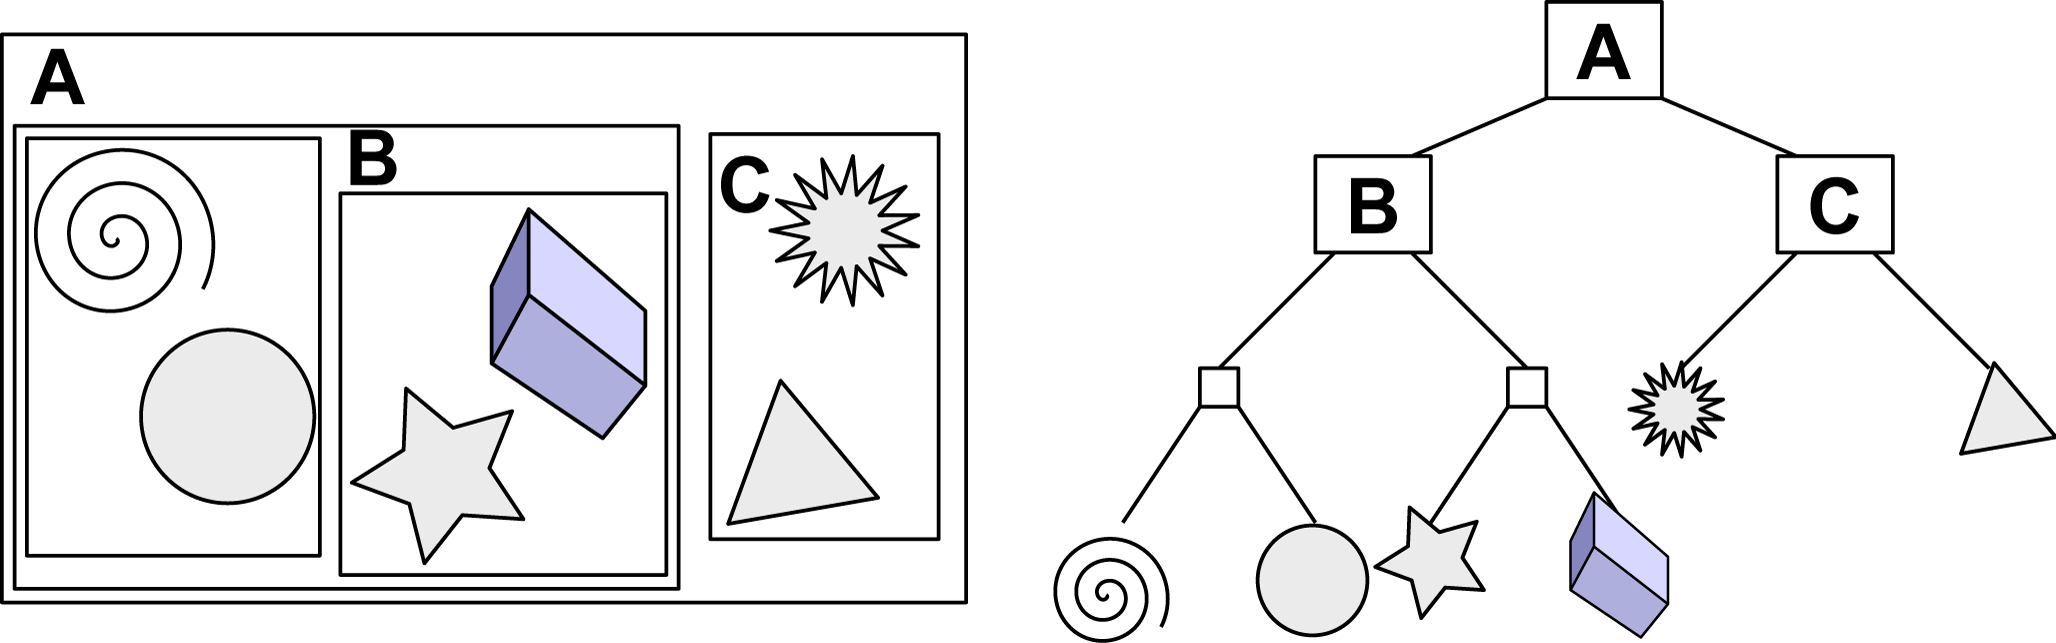
\includegraphics[width=\textwidth]{Figures/Simulations/bounding_volume_hierarchy.png}
    \caption{Example of 2D bounding volume hierarchy. 
             \textbf{Left:} the spacial relationship between solids and bounding volumes.
             \textbf{Right:} the intermediate nodes and the solids in the tree.
             From \cite{bounding_box_ref}}
    \label{fig:bvh_example}
\end{figure}
\par
Despite this, Chroma has some significant drawbacks.
Firstly, the code base is in python, which makes integration within the C++ GEANT4 simulation frameworks impractical.
Secondly, the inefficient handling of photon generation.
Copying information between the GPU and CPU should be minimised in order to increase performance.
Finally, although tessellation is adequate for some surfaces, many detectors are comprised of exclusively curved surfaces.
In order to achieve adequate accuracy, the number of primitives required begins to eliminate any gain in the processing speed.
\par
Inspired by Chroma, a separate project called Opticks was created \cite{Opticks_Paper_2017_ref,Opticks_CHEP_2019_ref,Opticks_CHEP_2021_ref}, which aims to tackle these limitations.
In the following section, the working principle of Opticks is described including adaptations and improvements made by the author for use within the LZ framework.

\subsection{Opticks}
\par
Whereas Chroma is built around CUDA, Opticks\footnote{Yes it is a confusing name} is built around NVIDIA OptiX \cite{nvidia_optix_paper_ref}, a ray tracing API.
As most ray-tracing algorithms require only a small set of operations, OptiX allows the user to build applications from a small set of CUDA programs.
These programs can define the ray generation, intersections with surfaces, camera characteristics and so on.
This means that a primitive can be correctly defined mathematically.
Additionally, more complex solids can be created by CSG as in GEANT4.
The primitives are described as boundaries \cite{real_time_collision_detection_ref}.
\par
Opticks has an important drawback compared to Chroma.
Chroma relies upon CUDA only and it is therefore not a significant challenge to port to OpenCL \cite{chroma_whitepaper_ref}.
This allows for non-NVIDIA GPU workflows.
However, for the foreseeable future, the performance will still lack significantly behind OptiX.
Additionally, all of the clusters which LZ currently use or plans to use contain NVIDIA GPUs, with the upcoming primary computing resource Perlmutter using NVIDIA A100 GPUs \cite{perlmutter_ref}.
\par
OptiX uses an acceleration structure which sorts primitives into spatial groups; essentially a tree of bounding boxes.
This is then used by a traversal algorithm to search for primitives that potentially intersect with a ray\footnote{OptiX provides acceleration to the geometrical intersection, not the intersection itself.}.
All details of the creation and traversing of the acceleration structures are handled internally by OptiX via user-defined bounding box programs.
The speed of the intersection calculations is related to the spatial grouping, and the creation of these groups remains a key research area in ray tracing \cite{NVIDIA_OptiX_GPU_Ray_Tracing_ACM_paper_ref,accelerated_bvh_ref}.
\par
Opticks is an open-source framework designed to convert GEANT4 geometry into an appropriate GPU form and perform photon simulations.
This includes the detector geometry and optical properties.
To allow for this, Opticks has ported the majority of GEANT4 primitives into CUDA equivalent ones \cite{Opticks_CHEP_2019_ref}.
Opticks converts the volume based geometry tree used by GEANT4 into a boundary based geometry model.
Each CUDA primitive is defined by intersection calculations which are based on those in \cite{real_time_collision_detection_ref} and a bounding box program.
All possible intersection directions are defined for each primitive; ray inside travelling outward, ray outside travelling inward.
The intersection decision of a solid is based upon \cite{CSG_Intersection_ref}, using a recursive algorithm.
However, OptiX does not allow for recursive intersection programs, so Opticks uses an always-left traversal method creating an iterative approach \cite{Opticks_Paper_2017_ref}.
\par
The resultant Opticks geometry tree is a set of binary trees with primitive leaves and operator nodes.
Practically speaking this is as NumPy serialised arrays, where each solid is defined by its own binary tree \cite{Opticks_Paper_2017_ref}, and these trees are indexed together based upon the structure.
These nodes are where rotations are defined.
Opticks navigates the binary tree via bitwise manipulation\footnote{parent $=i >> 1$, left child $= i << 1$, right child $(i<<1)+1$}.
This means that the tree height should be kept relatively low in order to reduce the number of nodes required to describe it.
As such, Opticks has a limit of 7 as $(1 << (7 + 1)) - 1 = 255$ corresponding to 255 nodes.
Opticks achieves this on trees which are not already of this height by attempting to balance them.
This is described in more detail in the following section.
\par
During the geometry conversion, Opticks attempts to highlight duplicate solids.
This way, when the geometry is uploaded to the GPU, the tree only needs to be uploaded once, and instancing is used which provides some memory saving \cite{Opticks_CHEP_2019_ref}.
Opticks also allows for geometry caching via NumPy serialisation \cite{Opticks_Paper_2017_ref} to avoid having to perform this conversion which is often computationally intensive more than once.
\par
In addition to the solids conversion, material and boundary properties are also translated as NumPy arrays which are indexed to which solids they refer to.
Separate CUDA programs handle the ray behaviour when influenced by these properties.

\par
In the next two sections, the translation of the LZ geometry is described along with initial performance metrics.
The proposed integration into the LZ simulation framework is discussed in-depth by the author in \cite{SEriksen_Opticks_CHEP_2021_ref}.

\subsection{LZ Geometry Conversion}
\par
In order to use the LZ geometry, it must first be extracted from GEANT4 where it is defined.
The simplest way to export a GEANT4 defined geometry is via a Geometry Description Markup Language (GDML) file \cite{GDML_USER_GUIDE_ref}.
GDML is a subset of XML which is designed to describe the geometry by describing a detector as a series of trees which correspond to the hierarchy of volumes \cite{GDML_USER_GUIDE_ref}.
A small excerpt of the LZ geometry GDML is shown below;
\begin{lstlisting}[backgroundcolor=\color{lightgrey},
                   language=XML, xleftmargin = 0.5cm]
<volume name="expHall_log0x1051db0">
  <materialref ref="vacuum0xea27f0"/>
  <solidref ref="expHall_box0x1152c20"/>
  <physvol name="subVol0x106c220">
    <volumeref ref="subVol_log0x1058260"/>
    <position name="subVol0x106c220_pos" unit="mm" x="0" y="0"
       z="1189.395000001"/>
  </physvol>
</volume>
\end{lstlisting}
In this extract, we can see the logical volume \textit{expHall\_log0x1051db0} which is filled with the solid box, \textit{expHall\_box0x1152c20}, that is made of a vacuum.
Inside this box a physical volume has been placed, \textit{subVol0x106c220} which contains the logical volume \textit{subVol\_log0x1058260}.
\par
The structure of the GEANT4 geometry is as PV/LV/PV/LV which means that if put into a geometry tree that isn't in the same style as GEANT4 it will require twice as many nodes to properly navigate it than is actually necessary.
As the PV contains the placement information of the LV and what sibling volumes it has, the PV information can be propagated into the LV and removed.

\par
The LZ detector contains a number of solids which are of sufficient complexity that the tree describing them is greater than 7 in depth.
These are typically unbalanced due to the way in which they were created in GEANT4, for example where a shape contains many holes (and therefore multiple subtractions).
These would likely have been implemented as one subtraction at a time from the primary solid.
A balanced approach would be to union subtractions together and then perform a single subtraction.
\autoref{fig:UnionSolidBinaryTree} describes a solid made up of 4 primitive solids, as an unbalanced and a balanced tree.
The balanced tree is less deep than the unbalanced tree and therefore is more efficient to navigate.
During the geometry conversion, Opticks recognises large trees and attempts to balance them via De Morgan's theorem \cite{Opticks_CHEP_2019_ref}.
De Morgan's theorem states that the complement of the union of two sets is the same as the intersection of their complements \cite{demorgans_law_ref}.
This results in a tree with only union, intersection operators and complemented primitives.
These complemented primitives are conceptually ``inside-out", but are implemented as just flipping the solid normal and classifying an intersection ``miss" becoming a volume ``exit".
\begin{figure}
\centering 
\begin{tikzpicture}[level distance=1.5cm,
  level 1/.style={sibling distance=3cm},
  level 2/.style={sibling distance=1.5cm}]
  \node {u}
    child {node {u}
      child {node {u}
        child {node {ps}}
        child {node {ps}}}
      child {node {ps}}}
    child {node {ps}};
\end{tikzpicture}
\begin{tikzpicture}[level distance=1.5cm,
  level 1/.style={sibling distance=3cm},
  level 2/.style={sibling distance=1.5cm}]
  \node {u}
    child {node {u}
      child {node {ps}}
      child {node {ps}}
    }
    child {node {u}
    child {node {ps}}
      child {node {ps}}
    };
\end{tikzpicture}
\caption{Binary tree representation of a simple solid comprised of the union (u) of 4 primitive solids (ps). \textbf{Left:} Unbalanced tree. \textbf{Right:} Balanced tree.}
\label{fig:UnionSolidBinaryTree}
\end{figure}
\par
This approach works for most unbalanced trees. 
However, it doesn't work for some of LZ's components.
For example, around the PMTs in the TPC exists a titanium plate and PTFE lining.
The titanium plate holds the PMTs in place, and the PTFE creates a reflective surface for photons on top of the titanium.
As the solids must have space for each PMT they are implemented as one solid with each hole subtracted out.
The tree for this (as defined in GEANT4) is shown in \autoref{fig:Opticks_unbalanced_shape}.
\begin{figure}
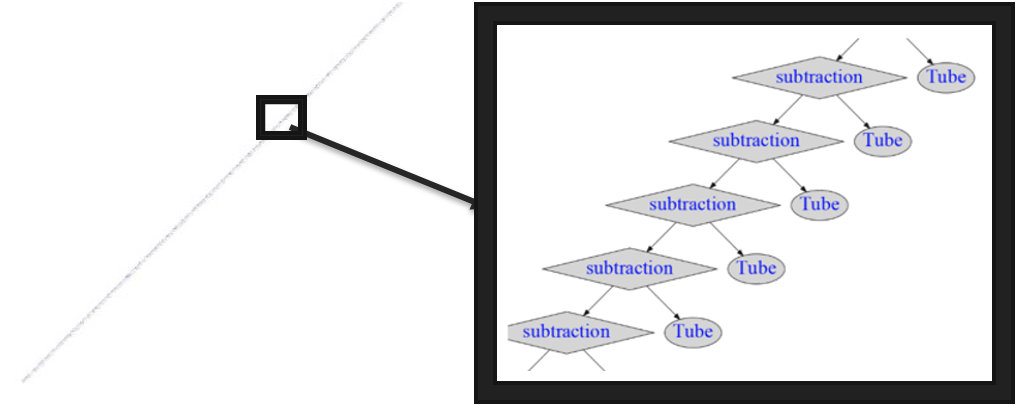
\includegraphics[width=\textwidth]{Figures/Simulations/unbalanced_ptfe.png}
\centering
\caption{Visual Representation of titanium top plate solid, comprised of a single G4Tube and 283 G4Tube subtractions. Kindly created by B. Krikler.}
\label{fig:Opticks_unbalanced_shape}
\end{figure}
For the top titanium plate this implementation would require $(1 << (253 + 1))-1 = 2^{254} - 1$ nodes, an impractically large number, making debugging near impossible due to memory requirements.
If perfectly balanced, this would still have a depth of 8, with 511 nodes which offers poor performance for the Opticks solid intersection calculation.
A method inspired by JUNO was adopted in order to handle this \cite{Opticks_CHEP_2021_ref}.
A primitive was created which defined the complex solid, so rather than being comprised of a CSG tree of multiple primitives, the tree became a single node of one complex primitive.
The basic creation process is shown in \autoref{fig:Opticks_PTFE_primative}.
In order to simplify the primitive code, the 3D shapes were reduced to 2D intersections.
3D is then introduced by duplicating the primitive and adding a Z-range in which the intersection needs to be evaluated.
Additional details of this approach can be found in \cite{optix_primitive_code_ref}.
Given the depth of these primitives, they are also likely a bottleneck in GEANT4 simulations, particularly the S2 light simulations mentioned in \autoref{sec:s2lightmap}.
In a branch of LZ code using GEANT4.10.6, 4 shapes were converted into G4MultiUnion solids which have built-in optimisation\footnote{At time of writing, LZ code uses GEANT4.10.3.p02 and this feature requiring unified solids was introduced in GEANT4.10.5 as an experimental feature} \cite{multiunion_ref}, with the computation time not increasing above 30-nodes\footnote{A boolean solid approach increases roughly linearly} \cite{multiunion_improvement_ref}.
The four shapes were the titanium plate and PTFE on the top and bottom PMT arrays in the TPC.
This adaptation decreased simulation time for S2 light by 56\%, a significant improvement.
\begin{figure}
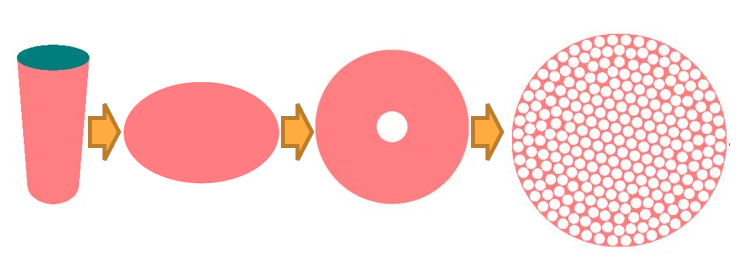
\includegraphics[width=0.7\textwidth]{Figures/Simulations/opticks_PTFE_primative.png}
\centering
\caption{Development stages for representing a 3D disc with multiple holes and a 2D disc with holes as defined within OptiX intersection program.}
\label{fig:Opticks_PTFE_primative}
\end{figure}

\par
The LZ geometry is comprised of in excess of 900,000 shapes, and although there is some duplication, this still leaves around 14,000 unique shapes.
Given the complications with solids such as the titanium plate, the scope of the conversion was limited to just the TPC and Skin.
This still leaves 9,000 unique shapes, which is 30-times greater than that of experiments which have previously used Opticks, such as JUNO and DayaBay \cite{Opticks_CHEP_2021_ref}.
Given this increased complexity many problems arose during the translation including GEANT4 optical properties used by LZ not having CUDA equivalent ones implemented in Opticks.
Where possible the LZ geometry was simplified to allow for progress to be made.
The most significant issue was with the GEANT4 ``groundfrontpainted" surface finish not having a CUDA implementation in Opticks.
This is where the surface of a volume is rough, so the normal of the surface is offset by some angle depending upon the micro-facet that the photon is incident upon and there can be internal Lambertian reflections \cite{optical_photons_in_geant4_ref}.
The author did develop this, but it was not used within the conversion here as it requires significant validation to ensure the results are comparable to the GEANT4 implementation.
Instead, wherever this optical surface occurred, it was replaced by the optical properties of another part of the detector, which was well-defined.
The completed TPC conversion is shown in \autoref{fig:OpticksLZTPC}.
\begin{figure}
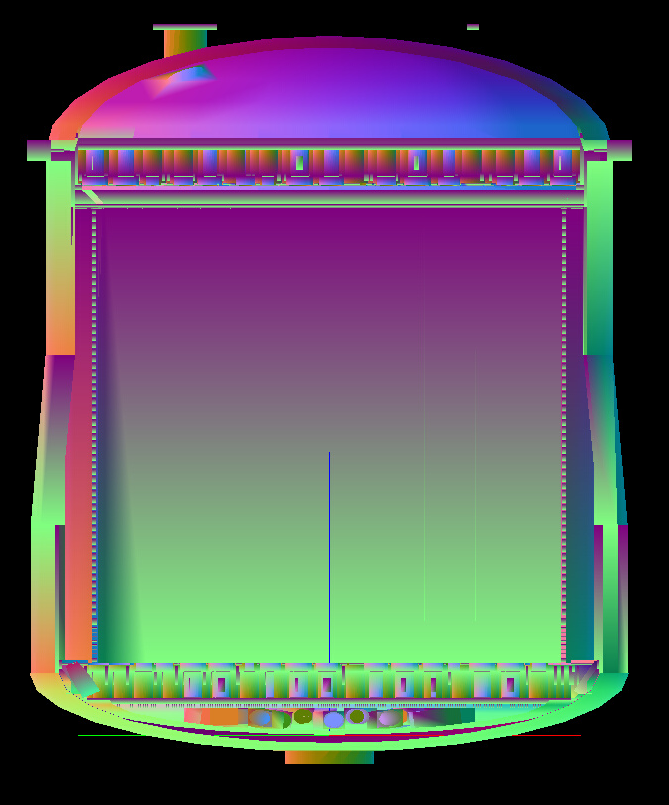
\includegraphics[width=8cm]{Figures/Simulations/LZ_In_Opticks.png}
\centering
\caption{TPC of LZ raytraced. Translated from Geant4 GDML file into a set of NumPy arrays using Opticks and viewed within Opticks via the OpenGL buffer.
The blue, green and red lines towards the bottom of the figure are the axes of the detector.}
\label{fig:OpticksLZTPC}
\end{figure}

\subsection{Performance and Outlook}
\par
LZ utilises multiple clusters across the globe.
In order to keep the computing environment constant, containers are used.
As such, as part of this work Opticks was containerised \cite{opticks_docker_ref} which also resulted in removing significant portions of legacy code and requirements from Opticks.
NVIDIA OptiX 6.5.0 and CUDA 10.2 were chosen as they were the newest fully supported versions within the Opticks framework.
Making use of NVIDIA container runtime to access the GPU, the container was successfully run - with graphics - on a range of computing resources.
This allowed for integration into the LZ framework to begin, the plan for which is described by the author in \cite{SEriksen_Opticks_CHEP_2021_ref,lz_status_with_opticks_ref}.
\par
As the geometry was cut down during the conversion and optical properties changed, the most valuable test that could be performed was a performance comparison to the S2 Light Map generation (\autoref{sec:s2lightmap}).
For this, 1,000,000,000 photons were generated as a ``photon bomb", a subset of which are shown in \autoref{fig:OpticksLZTPC_S1_Photons}.
On a Tesla T4 GPU, after a 4-minute initialisation time using the serialised geometry, 200,000 photons per second were generated and propagated.
This marks a 720x improvement over single-core Geant4 propagation where 277 photons per second were generated and propagated.
%and propagated for the S2 Light Map or 360x improvement over the expected gain when compared to GEANT4.
On the production clusters - such as Perlmutter - the performance is expected to increase.
This improvement highlights one of the reasons for choosing an OptiX-based approach rather than pure CUDA, as the improvement would have been closer to 200x such as was shown in \cite{chroma_presentation_ref}.
However, it still lags behind the improvement demonstrated using Opticks in \cite{Opticks_CHEP_2019_ref}, though this is primarily due to higher grade GPUs being used with RTX-cores.
With the newer NVIDIA OptiX 7.0.0+ \cite{NVidiaOptiX_7_ref}, the algorithms are expected to continue to increase in speed which should provide additional performance.
Unfortunately, the accuracy of this simulation has not been determined as that would require a major validation campaign of the optical processes, a process which needs to be performed before integration into the LZ simulation framework, but would have significantly delayed this thesis.


\begin{figure}
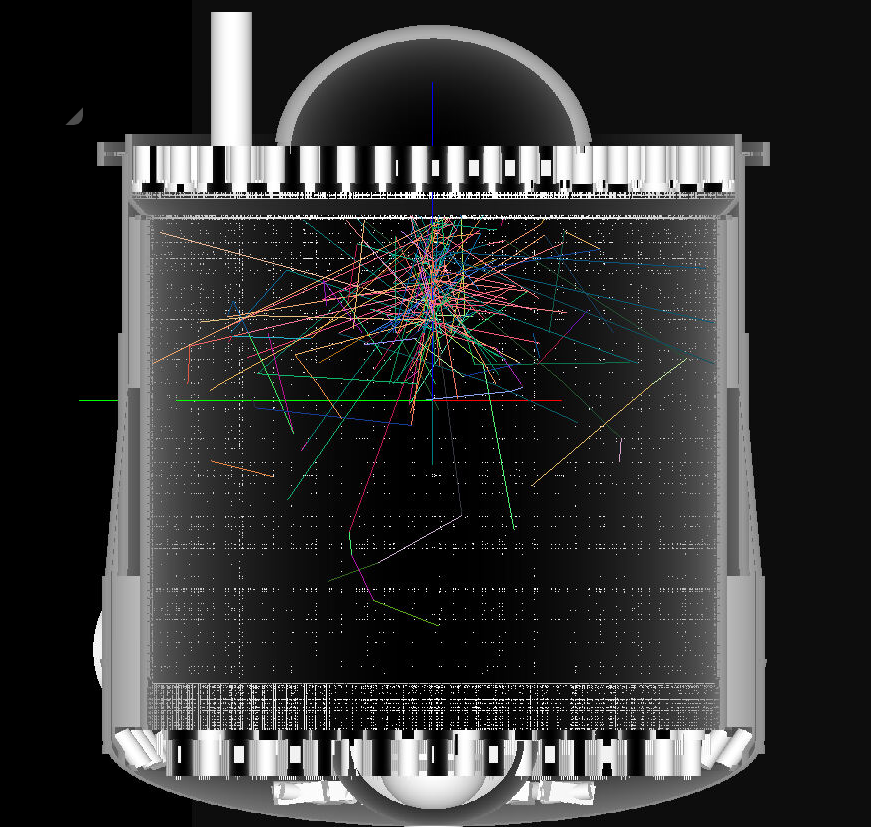
\includegraphics[width=10cm]{Figures/Simulations/LZ_S1_photons_In_Opticks.png}
\centering
\caption{TPC of LZ raytraced. Translated from Geant4 GDML file into NPY set using Opticks and viewed within Opticks via the OpenGL buffer.
The blue, green and red lines extended outside the OCV are the axes of the detector. After each reflection, a photon's colour has been set to change.}
\label{fig:OpticksLZTPC_S1_Photons}
\end{figure}